
\documentclass[10pt,a4paper]{report}
%\usepackage[latin1]{inputenc}
\usepackage[utf8]{inputenc}
\usepackage{amsmath}
\usepackage{amsfonts}
\usepackage{amssymb}
\usepackage{graphicx}
\usepackage{multicol}
\usepackage{tabularx}
\usepackage{tikz}
\usetikzlibrary{arrows,shapes,automata,petri,positioning,calc}
\usepackage{hyperref}
\usepackage{tikz}
\usetikzlibrary{matrix,calc}
\usepackage[margin=0.5in]{geometry}
% ---- power functions -----% 
\newcommand{\myvec}[1]{\ensuremath{\begin{pmatrix}#1\end{pmatrix}}}
\let\vec\mathbf

\providecommand{\norm}[1]{\left\lVert#1\right\rVert}
\providecommand{\abs}[1]{\left\vert#1\right\vert}
\let\vec\mathbf

\newcommand{\mydet}[1]{\ensuremath{\begin{vmatrix}#1\end{vmatrix}}}
\providecommand{\brak}[1]{\ensuremath{\left(#1\right)}}
\providecommand{\lbrak}[1]{\ensuremath{\left(#1\right.}}
\providecommand{\rbrak}[1]{\ensuremath{\left.#1\right)}}
\providecommand{\sbrak}[1]{\ensuremath{{}\left[#1\right]}}
%-------end power functions----%
\newenvironment{Figure}
  {\par\medskip\noindent\minipage{\linewidth}}
  {\endminipage\par\medskip}
\begin{document}
%--------------------logo figure-------------------------%
\begin{figure*}[!tbp]
  \centering
  \begin{minipage}[b]{0.4\textwidth}
    
\includegraphics[scale = 0.05]{iitlogo.jpg}
  \end{minipage}
  \hfill
  \vspace{5mm}\begin{minipage}[b]{0.4\textwidth}
\raggedleft  
\includegraphics[scale = 0.10]{nrc.png}\

  \end{minipage}\vspace{0.2cm}
\end{figure*}
%--------------------name & rollno-----------------------
\raggedright \textbf{Name}:\hspace{1mm} Chirag Shah\hspace{3cm} \Large \textbf{Assignment-5}\hspace{2.5cm} % 
\normalsize \textbf{Roll No.} :\hspace{1mm} FWC22053\vspace{1cm}
\begin{multicols}{2}

%----------------problem statement--------------%
\raggedright \textbf{Problem Statement:}\vspace{2mm}
\raggedright \\Construct the family of circles with fixed radius 5 units and center on the line y=2  .\\
\vspace{5mm}
%-----------------------------solution---------------------------
\raggedright \textbf{SOLUTION}:\vspace{2mm}\\

%---------given----------------%
\raggedright \textbf{Given}:\vspace{2mm}\\
Radius of a circle is \\\vspace{1mm}
\begin{align}
r = 5 
\end{align}
Center of circle lies on y=2\\ \vspace{1mm}
So,\\
\begin{align}
\beta=2
\end{align}

%-------------To find ------------------%
\textbf{To Find }\vspace{2mm}\\
Constructing the family of circles with different values of $\alpha$ \vspace{2mm}  \\ 
%--------------steps----------------------%
\textbf{STEP-1}\vspace{2mm}\\
Let r be the radius of circles which is given r=5 \\ \vspace{1mm}
Let $\vec{O}$ be the center of circle and the coordinates are,\vspace{1mm}
\begin{align}
\vec{O}=\myvec{
\alpha\\
\beta
}
\end{align} \vspace{2mm}
From given, we know that $\beta=2$ \\
So,\\
\begin{align}
\vec{O}=\myvec{
\alpha\\
2
}
\end{align} \vspace{2mm}
Let $\vec{X}$ be the any point on the circle \\\vspace{1mm}
\begin{align}
    \vec{X} = &r \myvec{
    cos\theta\\
    sin\theta
    }
\end{align}

\textbf{STEP-2}\vspace{2mm}\\
The equation of circle is given by, \\ \vspace{1mm}
\begin{align}
    \norm{\vec{X}-\vec{O}} = r 
\end{align}
\begin{center}
   $ \sqrt{(\vec{X}-\vec{O})^{\top}(\vec{X}-\vec{O})} = r $
\end{center}\vspace{5mm}

Squaring on both the sides \\ \vspace{2mm}
\begin{center}
( $ \sqrt{(\vec{X}-\vec{O})^{\top}(\vec{X}-\vec{O})} )^2 = r^2 $\\ \vspace{0.5cm}
$(\vec{X}-\vec{O})^{\top}(\vec{X}-\vec{O})=r^2$
\end{center}
Expanding the above equation,\\ \vspace{1mm}
\begin{align}
    \norm{\vec{X}}^2-2\vec{X}^{\top}\vec{O}+\norm{\vec{O}}^2=r^2
\end{align}
\textbf{STEP-3}\vspace{2mm}\\
Let $\theta$ be any angle from 0 to 2$\pi$\\ \vspace{1mm}
\begin{align}
    \theta \in [0,2\pi)
\end{align}
Let us assume, \\ \vspace{1mm}
\begin{align}
    \theta=\frac{2\pi}{3} 
\end{align}
Using equation (5) any point on circle   $ \vec{X}=\myvec{
    x\\
    y
    } $ is, \\ \vspace{1mm}
    Here ,\\  \vspace{2mm}
\begin{align}
    x=rcos\theta\\
    y=rsin\theta
\end{align}
\begin{align}
 \vec{X}=\myvec{
    -2.5\\
    4.3301
    } 
\end{align}
Let $\alpha$ be any values ranging from 0 to 10 with the incrementation of +2\\\vspace{1mm}

So, \\ \vspace{1mm}
\begin{align}
    \alpha = 0,2,4,6,8
\end{align}
If $\alpha=0$ ,\\ \vspace{1mm}
\begin{align}
    \vec{O}=\myvec{
    0\\
    2
    }
\end{align}
when $\alpha=2$ and so on till $\alpha=8$,\\ \vspace{1mm}
\begin{align}
    \vec{O}=\myvec{
    8\\
    2
    } 
\end{align}


\begin{center}
 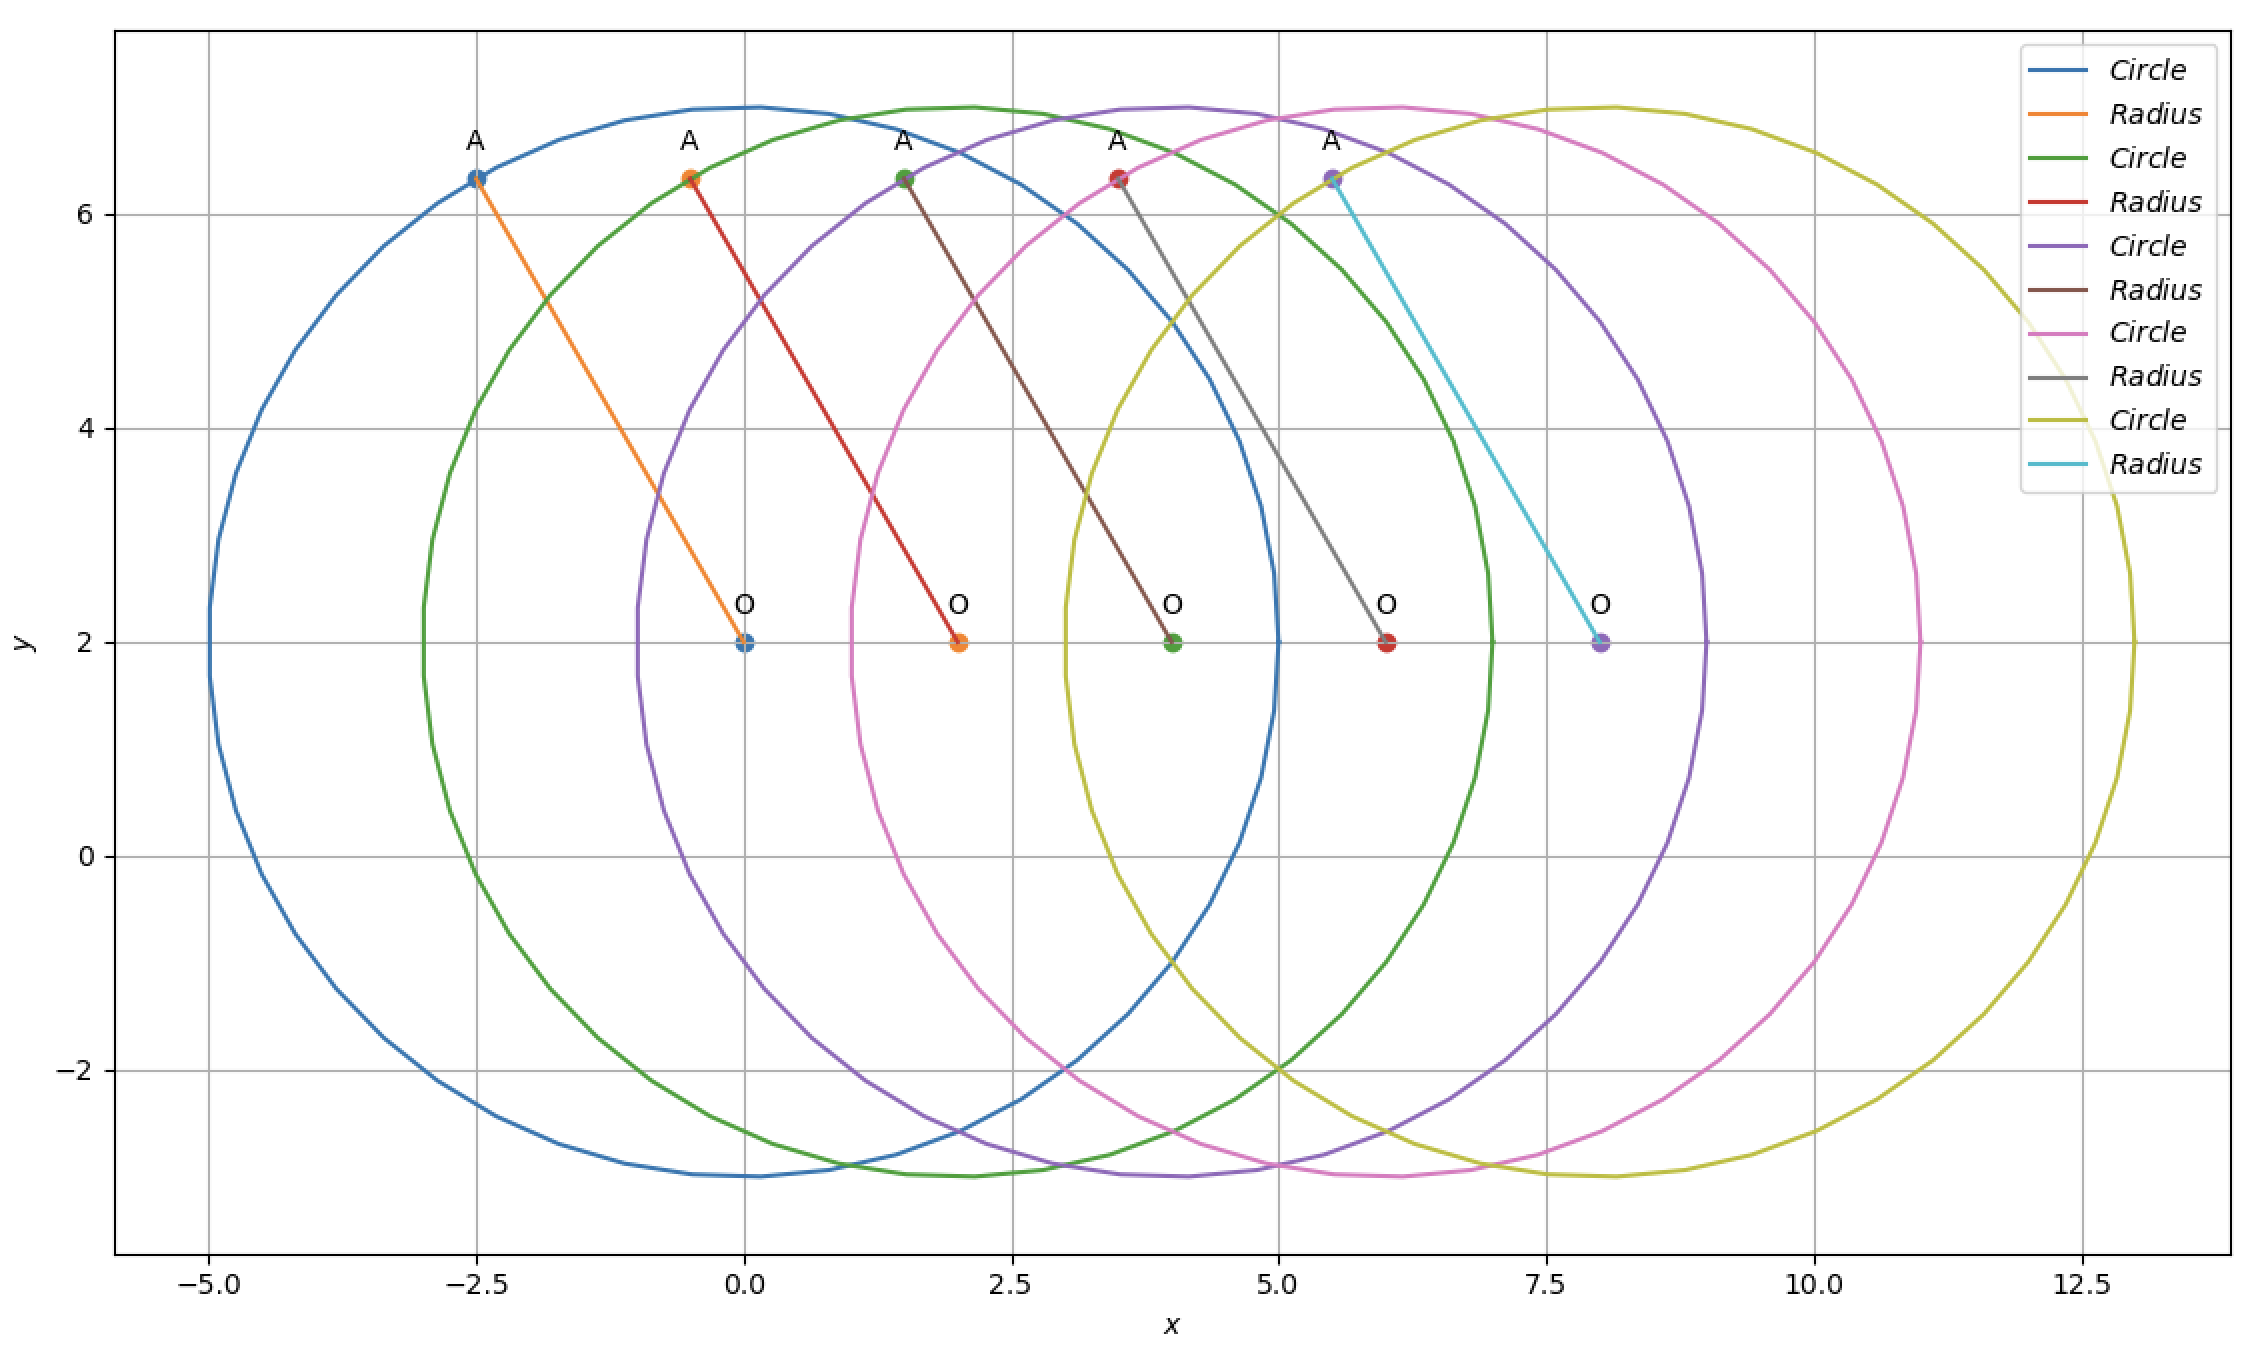
\includegraphics[width=0.5\textwidth]{circle.png}  
 \end{center}\vspace{1mm}
 
   

  
 \vspace{2mm} \textbf{Construction}
\begin{center}
\setlength{\arrayrulewidth}{0.5mm}
\setlength{\tabcolsep}{6pt}
\renewcommand{\arraystretch}{1.5}
    \begin{tabular}{|l|c|}
    \hline 
    \textbf{vertex} & \textbf{coordinates} \\ \hline
   $\vec{O}$ & $\myvec{
   \alpha\\
   2
   } $ \\\hline
   $\vec{X}$ & $\myvec{
   x\\
   y
   } $ \\\hline
      \end{tabular}
  \end{center}
  
\raggedright  Download the code \\
Github link: \href{https://github.com/chiragshah1244/FWC/blob/main/assignments/assignment_5/code/circle.py}{Assignment-5}.
  \end{multicols}
\end{document}